% Auto-generated by 04_additional_analysis.R — do not edit
% y > 0: Overreacts  |  y < 0: Underreacts
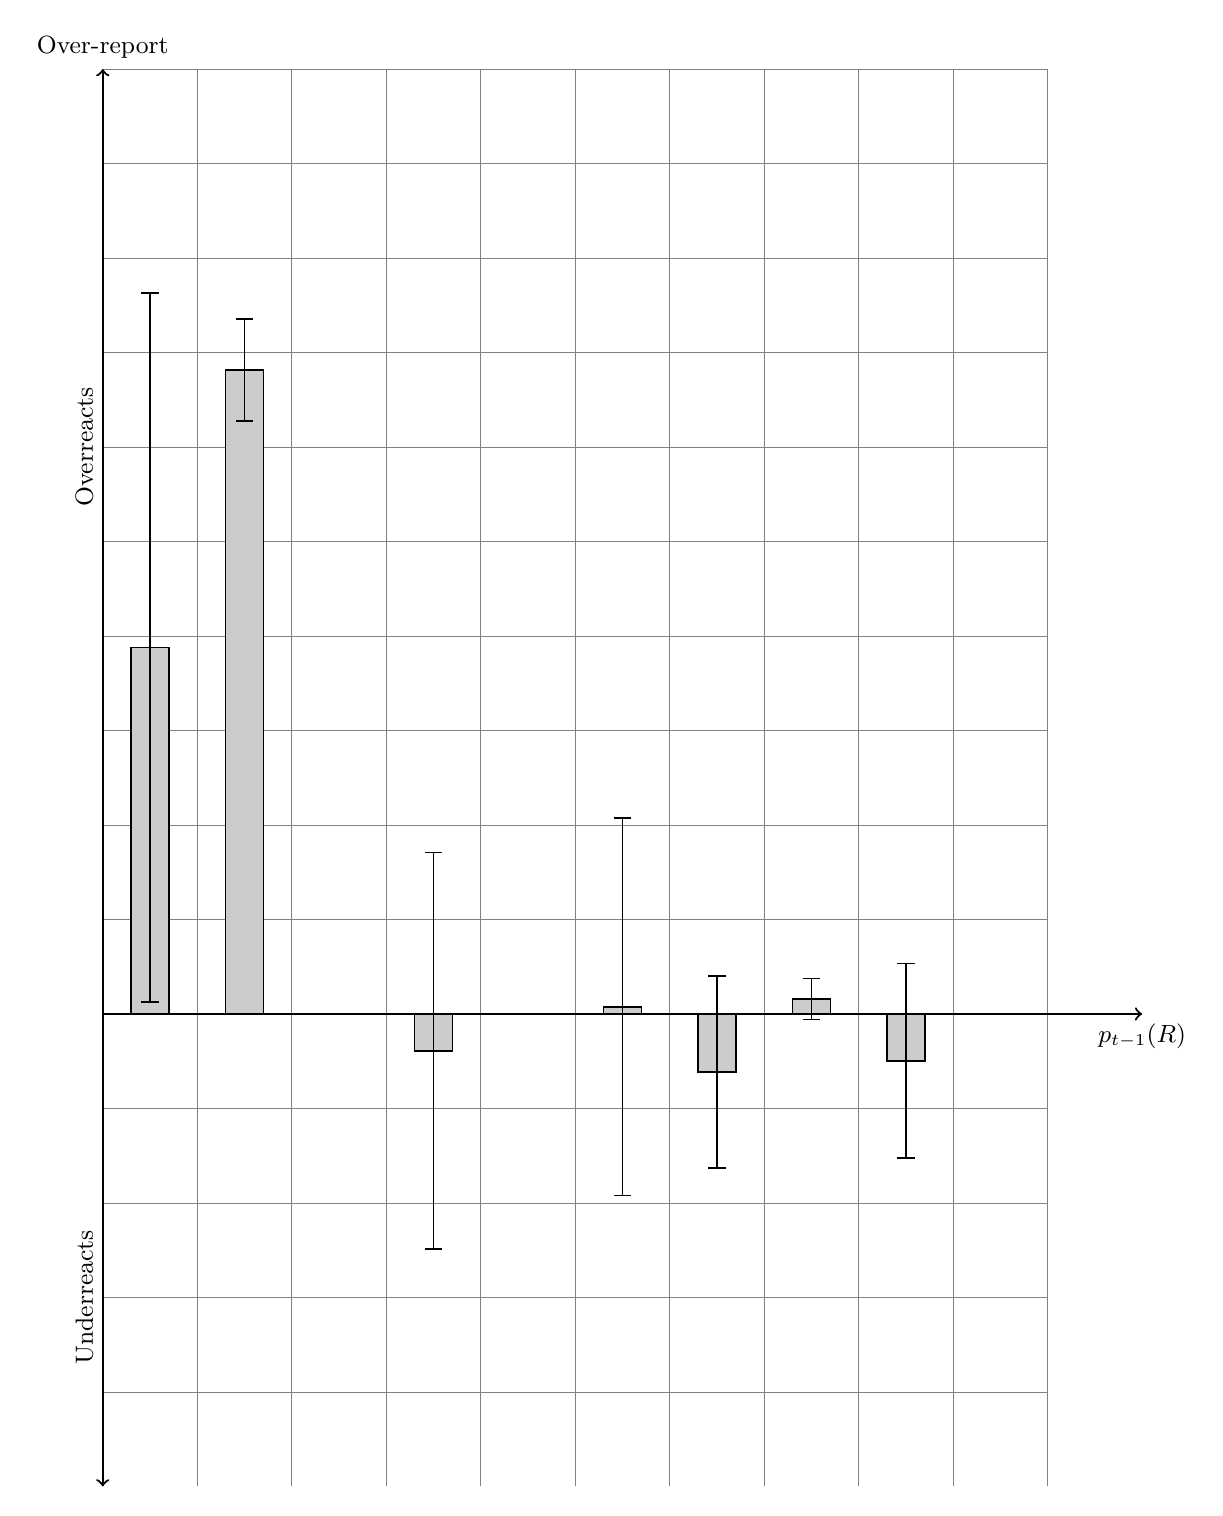
\begin{tikzpicture}[scale=12]
\draw[help lines,step=0.1] (0,-0.5) grid (1,1.0);
\filldraw[opaque,white!80!black] (0.03,0) rectangle (0.07,0.3879);
\draw[line width=0.6] (0.03,0) rectangle (0.07,0.3879);
\draw[line width=0.6,|-|] (0.05,0.0118) -- (0.05,0.7640);
\filldraw[opaque,white!80!black] (0.13,0) rectangle (0.17,0.6818);
\draw[line width=0.6] (0.13,0) rectangle (0.17,0.6818);
\draw[line width=0.6,|-|] (0.15,0.6270) -- (0.15,0.7365);
\filldraw[opaque,white!80!black] (0.33,0) rectangle (0.37,-0.0391);
\draw[line width=0.6] (0.33,0) rectangle (0.37,-0.0391);
\draw[line width=0.6,|-|] (0.35,-0.2499) -- (0.35,0.1717);
\filldraw[opaque,white!80!black] (0.53,0) rectangle (0.57,0.0077);
\draw[line width=0.6] (0.53,0) rectangle (0.57,0.0077);
\draw[line width=0.6,|-|] (0.55,-0.1931) -- (0.55,0.2085);
\filldraw[opaque,white!80!black] (0.63,0) rectangle (0.67,-0.0614);
\draw[line width=0.6] (0.63,0) rectangle (0.67,-0.0614);
\draw[line width=0.6,|-|] (0.65,-0.1637) -- (0.65,0.0410);
\filldraw[opaque,white!80!black] (0.73,0) rectangle (0.77,0.0157);
\draw[line width=0.6] (0.73,0) rectangle (0.77,0.0157);
\draw[line width=0.6,|-|] (0.75,-0.0069) -- (0.75,0.0383);
\filldraw[opaque,white!80!black] (0.83,0) rectangle (0.87,-0.0495);
\draw[line width=0.6] (0.83,0) rectangle (0.87,-0.0495);
\draw[line width=0.6,|-|] (0.85,-0.1532) -- (0.85,0.0543);
\draw[line width=0.8,->]  (0,0) -- (1.1,0) node[below] {\small{$p_{t-1}(R)$}};
\draw[line width=0.8,<->] (0,-0.5) -- (0,1.0) node[above] {\small{Over-report}};
\draw (0,0.60) node[above,rotate=90] {\small{Overreacts}};
\draw (0,-0.30) node[above,rotate=90] {\small{Underreacts}};
% ADD THEORY CURVE BELOW
\end{tikzpicture}
